% !TEX root = ../../main.tex
\section{Architecture}

Kafka's architecture revolves around a small set of primitives that compose into a
highly scalable, fault-tolerant messaging backbone.
Figure~\ref{fig:kafka-arch} shows the high-level cluster layout.

\begin{figure}[H]
  \centering
  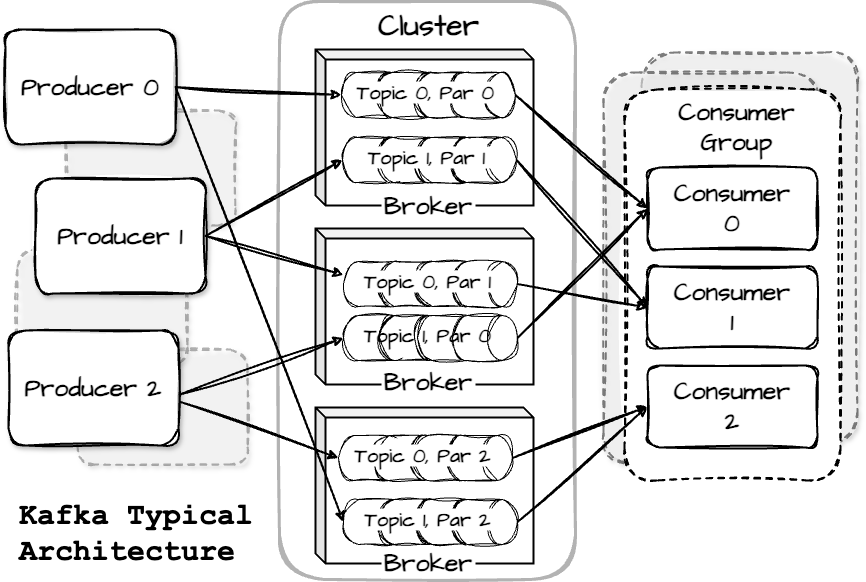
\includegraphics[width=0.92\textwidth]{image/kafka/kafka_architecture.png}
  \caption{Apache Kafka cluster architecture: producers, brokers, topics, partitions, and consumer groups.}
  \label{fig:kafka-arch}
\end{figure}

\subsection{Producer}

A \textbf{producer} is any client application that publishes records to one or more Kafka topics.
The producer library handles the following automatically:

\begin{itemize}
  \item \textbf{Partitioning} — the producer chooses a target partition for each record.
        If the record carries a \emph{key}, the partition is determined by \texttt{hash(key) \% numPartitions},
        guaranteeing that all records with the same key land in the same partition (and are therefore totally ordered).
        Without a key, records are distributed round-robin across partitions for even load balancing.
  \item \textbf{Batching} — records destined for the same partition are accumulated in an in-memory buffer
        (\texttt{batch.size}) and sent together after a short delay (\texttt{linger.ms}),
        dramatically improving network throughput at the cost of a small, tunable latency.
  \item \textbf{Compression} — entire batches can be compressed with GZIP, Snappy, LZ4, or ZSTD
        before transmission, reducing both network bandwidth and broker disk usage.
  \item \textbf{Acknowledgement modes (\texttt{acks})} — the producer waits for an acknowledgement
        from the broker before considering a write successful:
    \begin{itemize}
      \item \texttt{acks=0}: fire-and-forget — maximum throughput, zero durability guarantee.
      \item \texttt{acks=1}: leader acknowledges — fast, but data may be lost if the leader crashes before replicating.
      \item \texttt{acks=all}: all in-sync replicas (ISR) acknowledge — strongest durability, moderate latency cost.
    \end{itemize}
  \item \textbf{Idempotent producer} — when enabled (\texttt{enable.idempotence=true}), the broker
        deduplicates retried batches using a sequence number, providing exactly-once write semantics.
\end{itemize}

\subsection{Broker}

A \textbf{broker} is a Kafka server process responsible for persistently storing records and
serving read/write requests from producers and consumers.

\begin{itemize}
  \item Each broker stores a subset of the cluster's partition \textbf{replicas}.
        For every partition, one broker is the \textbf{leader} (handles all reads and writes);
        the remaining brokers in the ISR are \textbf{followers} that passively replicate from the leader.
  \item If a leader broker crashes or becomes unreachable, Kafka elects a new leader from the ISR set
        automatically — typically within seconds — with no manual intervention required.
  \item Records are written to a partition as an \textbf{append-only segment log} on local disk.
        Sequential I/O (rather than random seeks) is the primary reason Kafka achieves very high write throughput
        even on commodity spinning disks.
  \item A healthy production cluster typically runs \textbf{3–5 brokers}, with a replication factor of 3,
        tolerating up to 2 simultaneous broker failures without data loss.
\end{itemize}

\subsection{Topic}

A \textbf{topic} is a named, logical channel to which producers append records and from which
consumers read.
Think of it as a database table, except that:

\begin{itemize}
  \item Records are \textbf{immutable} once appended — they cannot be updated or deleted (only expired).
  \item \textbf{Retention} controls how long records survive on disk.
        Time-based retention (e.g.\ 7 days) deletes old segments once they age out;
        size-based retention deletes once the topic exceeds a configured byte limit.
  \item \textbf{Log compaction} is an alternative mode that retains the latest record for each key indefinitely,
        making the topic behave like a key-value changelog — ideal for CDC (Change Data Capture) streams.
\end{itemize}

\subsection{Partition}

Each topic is divided into one or more \textbf{partitions}, which are the fundamental
unit of parallelism and ordering in Kafka.

\begin{itemize}
  \item A partition is an \textbf{ordered, immutable sequence} of records.
        Each record is assigned a monotonically increasing \textbf{offset} upon arrival,
        uniquely identifying its position within that partition.
  \item Ordering guarantees are \emph{within} a partition only.
        If global ordering matters (e.g.\ all events for a single user), the application must
        route those events to the same partition via a consistent key.
  \item The number of partitions in a topic is the main knob for scaling:
        more partitions = more parallel writes by producers and more parallel reads by consumers.
        However, partitions cannot be reduced once created, and too many partitions increase
        leader-election overhead, so the partition count requires careful planning.
  \item Each partition replica is stored as a sequence of \textbf{segment files} on the broker's disk,
        with an index file for fast offset lookups.
\end{itemize}

\subsection{Consumer and Consumer Group}

A \textbf{consumer} reads records from a partition by \emph{polling} the broker and
tracking its current position via a \textbf{committed offset}.

\begin{itemize}
  \item \textbf{Pull model} — consumers pull data at their own pace.
        Kafka never pushes records, so a slow consumer does not apply back-pressure to the broker
        or to other consumer groups reading the same topic.
  \item \textbf{Offset management} — the consumer commits the offset of the last record it has
        successfully processed to a special internal topic (\texttt{\_\_consumer\_offsets}).
        On restart, it resumes from the committed offset, preventing both data loss and duplicate processing.
        Commits can be \emph{automatic} (periodic) or \emph{manual} (after the application confirms success).
  \item \textbf{Consumer group} — a logical group of consumer instances that jointly consume a topic.
        Kafka assigns each partition to \emph{exactly one} member of the group at any point in time,
        distributing load evenly.
        Multiple independent groups can consume the same topic simultaneously, each with its own offset cursor —
        this is how Kafka achieves fan-out without duplicating data.
  \item \textbf{Rebalancing} — when a consumer joins or leaves the group (or a partition count changes),
        the group coordinator triggers a rebalance that reassigns partitions among the active members.
        Modern Kafka clients support \emph{cooperative rebalancing} to minimise disruption during the handover.
  \item \textbf{Parallelism rule} — the maximum useful parallelism for a consumer group equals the number
        of partitions in the topic; adding more consumers than partitions leaves the extra consumers idle.
\end{itemize}
